\chapter{Introduction}

The field of language modeling has undergone a dramatic transformation in recent years. In 2021, the release of GPT-3, a language model with \textbf{175 billion parameters}, marked a significant milestone for the field of natural language processing (NLP). GPT-3 set a new standard for performance on a wide range of language understanding tasks, in many cases achieving or surpassing human-level capabilities \citep{brown2020gpt3}. At the time, its unprecedented scale drew comparisons to the 86 billion neurons in the adult human brain \citep{azevedo2009neurons} and underscored the pace at which artificial systems were beginning to mirror the complexity of biological systems.

In just four years, the scale and ambition of language models have grown exponentially. Although the exact specifications of GPT-4 remain undisclosed, it is widely estimated to contain approximately 1.8 trillion parameters. Similarly, Google's Gemini Ultra has been reported at around 1.5 trillion. These figures reflect an order-of-magnitude leap in model size compared to GPT-3 and highlight an accelerating trend toward ever-larger architectures at the frontier of AI research.

This rapid scaling has delivered tangible gains in capability. Tasks once considered aspirational, such as reasoning over long contexts \citep{lewis2020retrieval}, synthesizing code \citep{chen2021evaluating}, or interpreting multi-step instructions \citep{wei2022chain}, have become increasingly tractable for these large models. Performance gains are evident across standard evaluations including MMLU \citep{hendrycks2021mmlu}, BIG-bench \citep{srivastava2023bigbench}, and HellaSwag \citep{zellers2019hellaswag}, with state-of-the-art models demonstrating consistent improvement since 2021.

However, this order-of-magnitude leap in scale raises an important question: are these advances in NLP reflective of better language modeling techniques, or simply the result of building larger models? 

This question becomes even more pertinent when examining performance trends over time. As \cref{fig:model_size_vs_performance} illustrates, there exists a notable divergence in the language modeling landscape. While large models demonstrate consistent improvement year after year, smaller models of fixed size (~100M parameters) have plateaued despite advances in training techniques. This trend suggests that recent progress may be driven more by scaling than by fundamental advances in efficiency.

\begin{figure}[htbp]
    \centering
    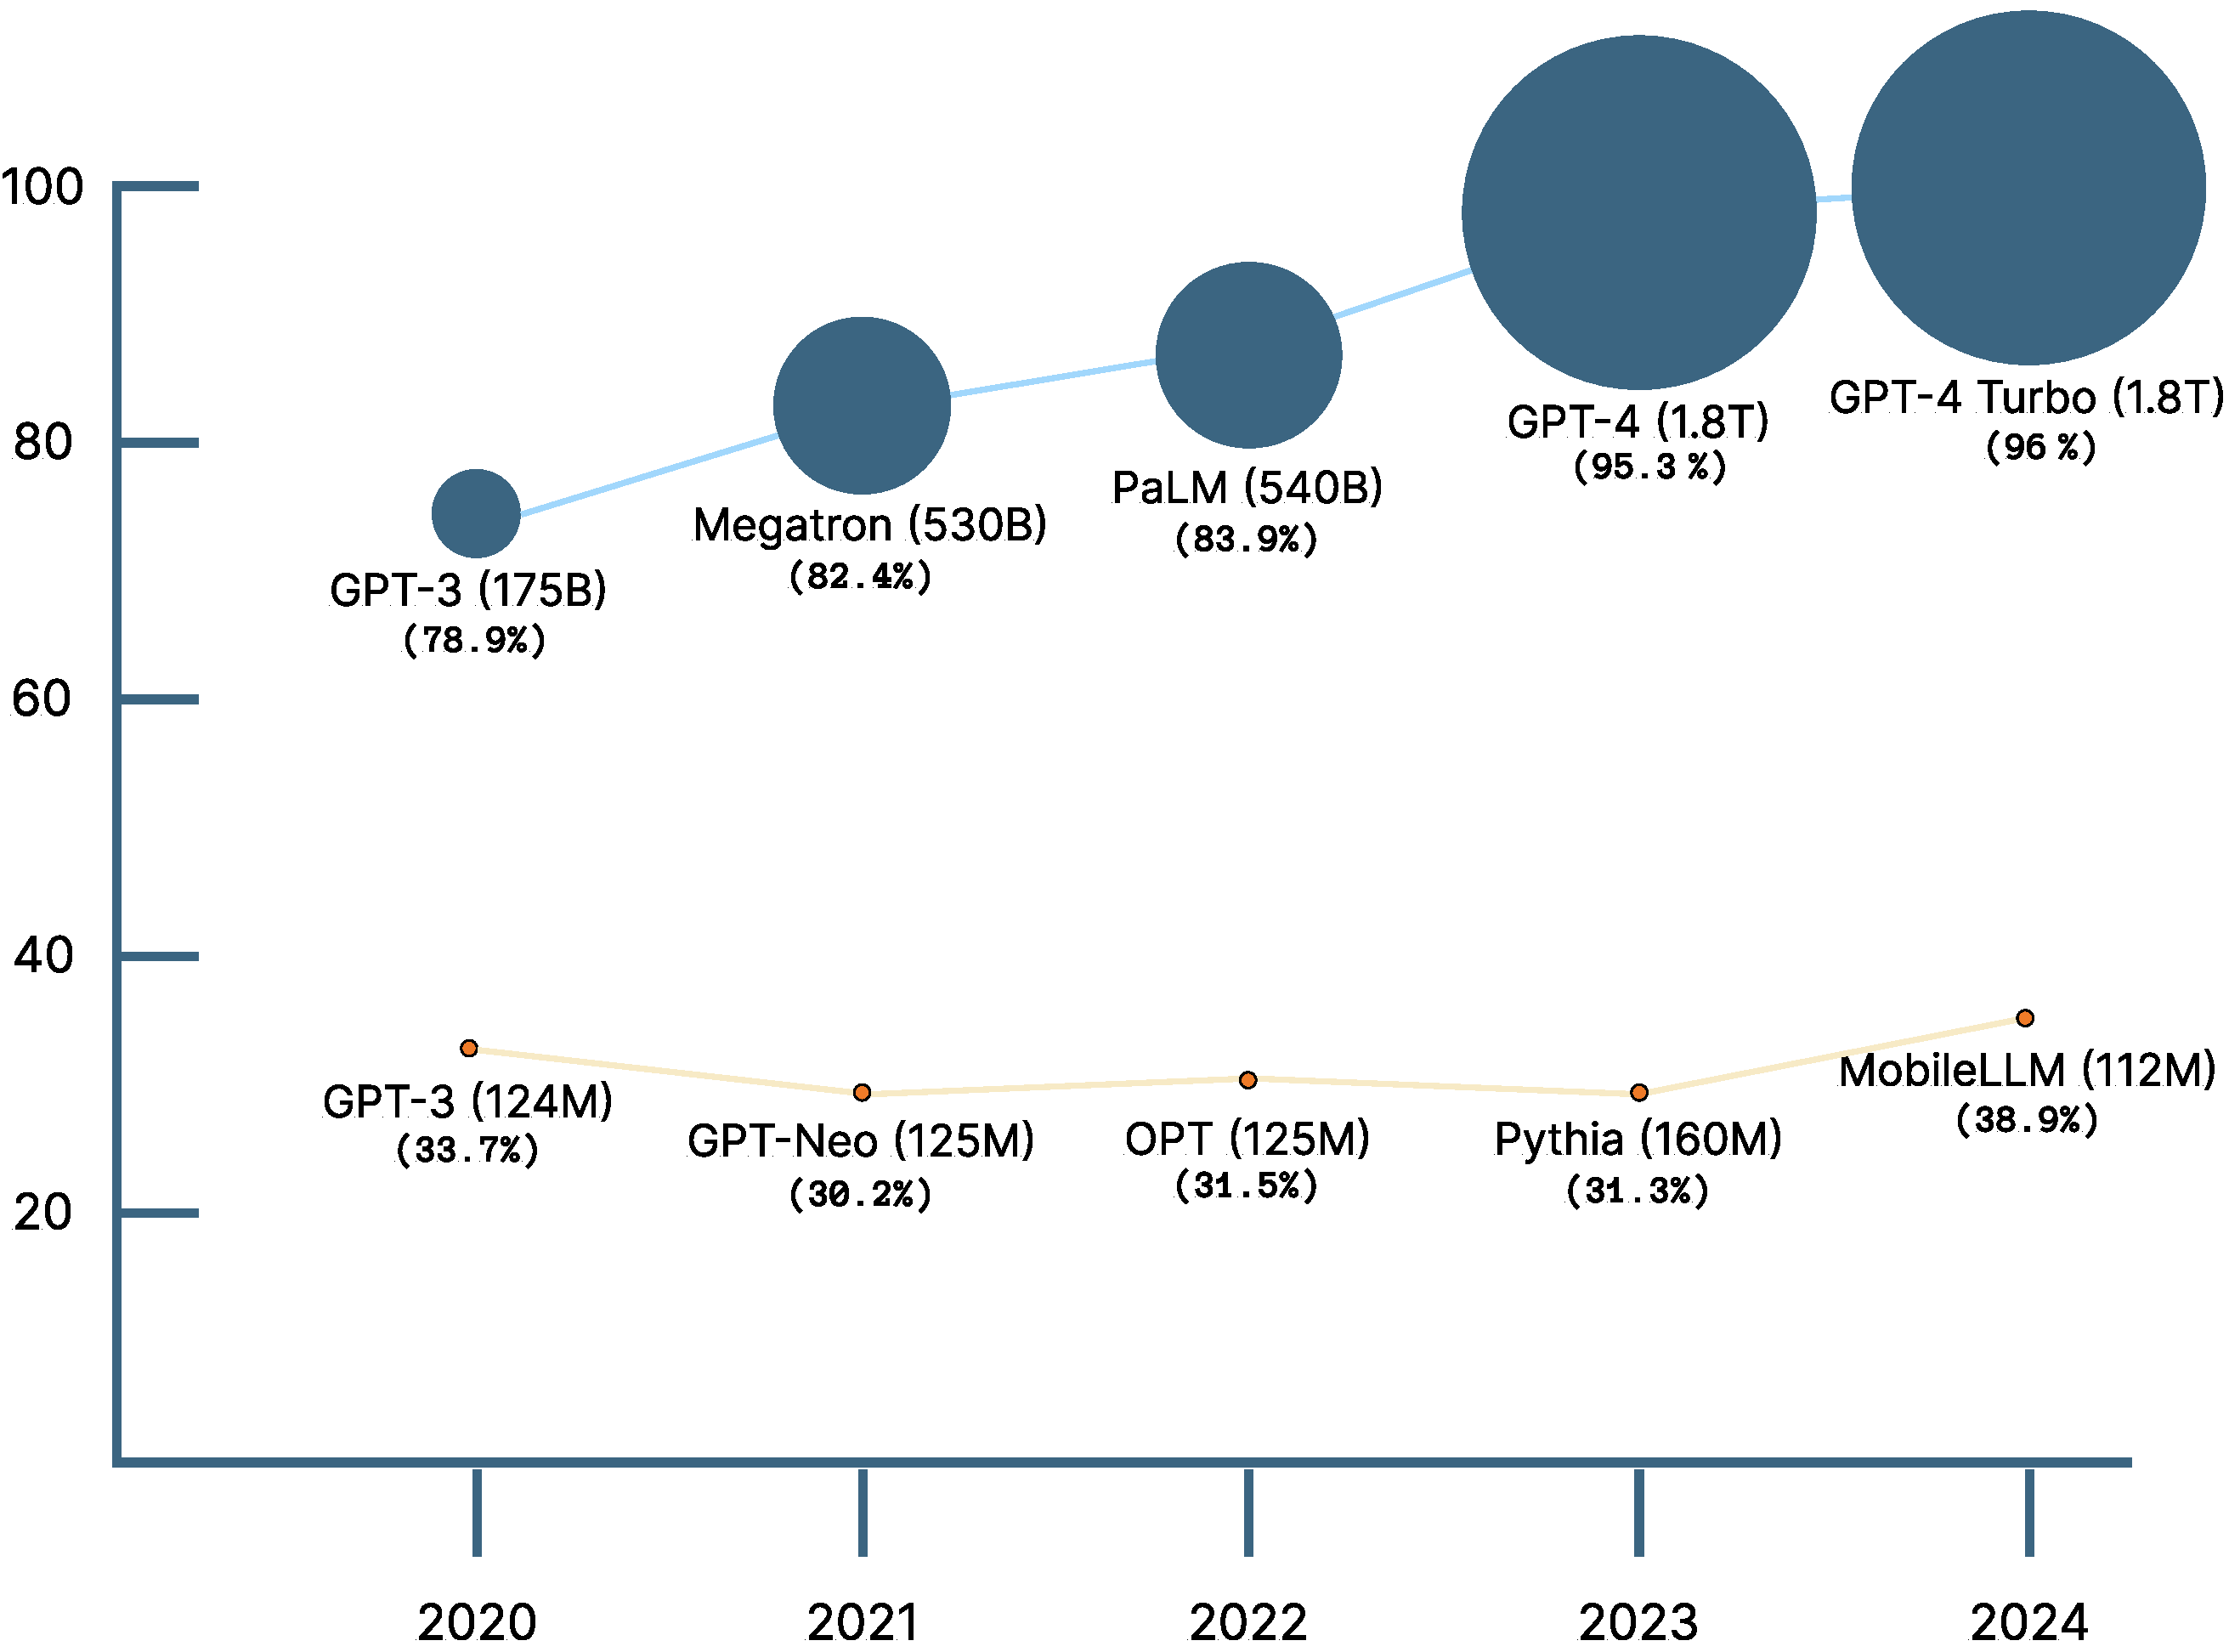
\includegraphics[width=0.8\textwidth]{chapters/introduction/figures/lm_performance_comparison.pdf}
    \caption{Performance of small and large language models on the HellaSwag dataset over time. The plot reveals a striking divergence: while \textbf{\textcolor[HTML]{37718E}{large}} models show consistent improvement, \textbf{\textcolor[HTML]{FF7F11}{small}} models have plateaued despite advances in training techniques.}
    \label{fig:model_size_vs_performance}
\end{figure}

This insight extends beyond academic interest. While frontier models dominate public and industrial attention, small language models remain vital for several reasons. %They are not only essential for deployment in resource-constrained environments—such as mobile devices and edge computing—but also play a critical role in enabling transparency, reducing costs, and improving accessibility across a wider range of applications.

\section*{Why Do Small Models Matter?}

% We should also probably define what we mean by small models.

The rapid scaling of language models has brought about remarkable capabilities, but it has also surfaced a host of challenges and risks \citep{bommasani2021foundation}. Small language models, which are compact, efficient, and accessible, offer a promising counterbalance.

\paragraph{Large models introduce significant societal risks.} As enumerated by the Stanford Center for Research on Foundation Models \citet{bommasani2021foundation}, these include the potential for generating disinformation and misinformation at scale, amplifying biases and discrimination present in training data, and memorizing and regurgitating sensitive or copyrighted content. The sheer scale of these models also raises concerns about labor displacement, environmental impact, and the creation of single points of failure, as a widely deployed model that is compromised could have cascading negative effects across all downstream applications. Notably, the authors highlight that the risks associated with large models are not just technical but also social, as they can entrench power in the hands of a few organizations and make it harder to adapt models to specific, local needs.

\paragraph{Large models pose serious environmental sustainability challenges.} As a result, researchers have increasingly emphasized energy efficiency as a core evaluation metric, on par with traditional measures like accuracy \citep{schwartz2020greenai}. Studies have quantified the financial and carbon costs of training state-of-the-art NLP systems, revealing orders-of-magnitude differences between large and small models \citep{strubell2019energy}. For example, a modest increase in translation accuracy can result in a dramatic rise in compute cost. Tools like the ML Emissions Calculator \citep{lacoste2019quantifying} and systematic reviews of emissions factors \citep{luccioni2023counting} have made it clear that model size, hardware, and training recipes all play a role in determining the environmental footprint of machine learning. Transformer-based models, in particular, are among the most energy-intensive, especially when techniques like neural architecture search are used. Benchmarks such as HULK \citep{zhou2021hulk} have compared pretrained models' energy efficiency, showing that smaller models are far more efficient in both time and cost. Furthermore, the location where models are trained can significantly affect emissions, and sparsely activated models can be much more energy-efficient than their dense counterparts \citep{patterson2021carbon}. The overall trend is clear: smaller models are more sustainable, and their adoption is crucial for reducing AI's environmental impact.
%TODO: Last two sentences are a bit of a non sequitur.

\paragraph{Data privacy and memorization risks are heightened in large models.} Research has shown that neural networks, especially large ones, can memorize and regurgitate rare or sensitive training data \citep{feldman2020neural, carlini2019secret}. Follow-up studies have demonstrated that memorization increases with model size and data duplication, and have introduced methods to extract such memorized content from models without access to the original training set \citep{carlini2021extracting, carlini2022quantifying}. Comprehensive surveys have categorized the security and privacy risks of large language models, including inference-time leakage, adversarial vulnerabilities, and systemic risks from centralization \citep{yao2024privacysurvey}. Larger models are more likely to leak personally identifiable information, especially when trained on duplicated or low-diversity data \citep{huang2022large, neel2023privacy}. Mitigation strategies such as differential privacy \citep{dwork2006calibrating} and federated learning \citep{mcmahan2017communication} have been proposed, but these often come with trade-offs in model utility. Scaling laws for memorization further confirm that as models grow, so does their propensity to memorize and leak sensitive information \citep{lu2024scaling, biderman2023emergent, kiyomaru2024comprehensive}. In contrast, smaller models, with less capacity to memorize, offer a more privacy-preserving alternative—especially when combined with privacy-focused training techniques.

\paragraph{Small models are uniquely suited for on-device and edge deployment.} Efficient inference with limited memory is essential for running language models on consumer hardware, and recent work has shown that even models with billions of parameters can be optimized for such use cases \citep{alizadeh2024llm}. Sub-billion parameter models are particularly important for energy-efficient, on-device applications, as demonstrated by \citet{liu2024mobilellm}. Earlier advances in mobile-friendly architectures, such as MobileNets \citep{howard2017mobilenets} and EfficientFormer \citep{li2022efficientformer}, laid the groundwork for efficient models in both vision and language domains. The importance of energy-proportional memory for datacenter and mobile applications has also been highlighted \citep{malladi2012towards}. These advances make it possible to run language models in privacy-sensitive, resource-constrained, or offline settings, broadening the reach and utility of AI.

\paragraph{Interpretability and scientific understanding are further reasons to prioritize small models.} The internal mechanisms of transformers and other neural architectures are more tractable in smaller models, making them better testbeds for developing scientific understanding \citep{elhage2021mathematical, elhage2022toy, bircken2023monosemanticity, anthropic2023components}. Tools such as influence functions are easier to apply at small scale, and the "manifold hypothesis" suggests that smaller models are ideal for probing the structure of neural representations \citep{olah2014manifolds}. Progress in understanding larger models often begins with insights gained from studying their smaller counterparts.

\paragraph{Finally, the democratization and accessibility of language technology depend on the availability of small, open models.} The cost of training and deploying large models is rising rapidly, with the financial and hardware requirements putting them out of reach for most organizations and individuals \citep{cottier2024rising, sharir2020cost}. Minimal, well-documented implementations like nanoGPT \citep{karpathy2023nanogpt} and Pico \citep{diehlmartinez2025pico} make language modeling accessible to a broader community, supporting education, experimentation, and innovation. By lowering the barrier to entry, small models enable more researchers, organizations, and communities to participate in the development and application of language technologies.

% In summary, small language models matter because they are more sustainable, privacy-preserving, interpretable, and accessible. They offer a practical and ethical path forward for language technology, especially as the risks and costs of large-scale models continue to mount.

\section*{Research Objectives}

This thesis aims to explore how small language models can be trained more efficiently and effectively, emphasizing principled approaches over brute-force scaling. The work is structured around two central research objectives:

\begin{quote}
    \textbf{Research Question 1: Can insights from human language acquisition be leveraged to develop more principled and effective training paradigms for small language models?}
\end{quote}

Despite recent advances in architecture design and compression techniques, small models continue to lag behind their larger counterparts. Yet they are critical for real-world deployment due to their efficiency, interpretability, and accessibility.

A persistent challenge in this area is that many of the methods proposed to improve small models, ranging from ad hoc architectural tweaks to various forms of regularization or data augmentation, often lack a strong scientific foundation. Progress is frequently incremental and difficult to interpret; new techniques sometimes offer only marginal gains or fail to generalize beyond specific benchmarks. Without a principled framework or guiding thesis, it becomes challenging to systematically understand what works, why it works, and how to build on prior results in a cumulative way.

One promising guiding thesis is to look to human language acquisition for inspiration. While today's large language models are trained on trillions of tokens, a typical 13-year-old human has been exposed to only around 100 million words. This dramatic discrepancy highlights a key inefficiency in current training paradigms and suggests an opportunity: do strategies that work well for the human brain also confer advantages in artificial models? And can cognitive science offer a roadmap toward more efficient, adaptable, and robust language modeling?

By grounding small model training in insights from human cognition, this thesis seeks to move beyond ad hoc heuristics and toward a more principled, theory-driven foundation. Rather than treating efficiency as an afterthought, the goal is to understand how cognitive strategies, such as curriculum learning, inductive biases, and compositional generalization, might translate into practical improvements in model design and training. In doing so, this work aims to bridge the gap between machine learning and cognitive science, offering not only empirical results but also conceptual tools for building small language models that are both efficient and robust.

To complement this exploration of training strategies, the second research objective focuses on understanding the learning dynamics of small models more deeply and rigorously.

\begin{quote}
    \textbf{Research Question 2: How can we more quantitatively understand how small models learn and what makes them different from large models?}
\end{quote}

Improving training efficiency is only part of the broader challenge. Equally important is developing a deeper understanding of the underlying learning dynamics that drive how language models learn: How can we quantitaively study the learning process of language models? And how can we characterize the differences in learning between small and large models in a systematic, interpretable way? These questions demand not just better engineering, but a more scientific, principle-driven approach to model understanding.

In recent years, efforts to improve small language models have often relied on empirical heuristics, ranging from architecture tweaks to training tricks, that offer marginal gains but lack deeper explanatory power. This trial-and-error mindset can obscure the mechanisms behind success and makes it difficult to generalize progress across tasks, model sizes, or domains. Small models, by contrast, offer an opportunity to observe the learning process more transparently. Their smaller size makes them easier to study, as they are less complex, faster to train, and more accessible for detailed analysis.

To make progress, we must go beyond outcome-based benchmarks and focus on the learning process itself: how knowledge is acquired, how model capacity is structured and used, and how different factors shape convergence dynamics. Small models provide a unique lens for this investigation not only because they are easier to analyze, but because their behavior often reveals the underlying structure of learning in ways large models conceal.

This research objective, therefore, is grounded in the belief that meaningful progress in model development must be built on a deeper understanding of the learning process itself. By focusing on measurable, interpretable properties of training, such as model convergence dynamics and representational capacity, we can begin to articulate a more cumulative and principled science of language model development.

\section*{Thesis Overview}

This thesis is organized into two parts, reflecting the two research threads:

\subsection*{Part I: Cognitive Insights for Efficient Training (Chapters 2–4)}

\begin{itemize}

    \item \textbf{Chapter 2:} \emph{The Evolution of Language Modeling: Foundations, Scale, and Efficiency} offers a comprehensive overview of the development of language modeling, tracing its trajectory from early statistical approaches to contemporary neural methods. The chapter begins with foundational concepts, including n-gram models, and progresses through key milestones such as neural language models, word embeddings, and the advent of attention mechanisms. It analyzes how large-scale language models have transformed the field, introducing emergent capabilities and shifting the research landscape. At the same time, it highlights the increasing relevance of smaller, more efficient models. The chapter reviews major strategies for enhancing the efficiency of small models, encompassing architectural innovations, optimization techniques, and data calibration methods. It concludes by drawing connections between machine learning and cognitive science, considering how insights from human language acquisition can inform more principled model development, especially in resource-constrained environments.


    \item \textbf{Chapter 3:} \emph{Language Learning with Limited Data: Insights from Human Development for Curriculum Design}  
    explores a systematic investigation of curriculum learning strategies inspired by human language acquisition, focusing on their application to small language models. The work is motivated by the striking efficiency of human language learning compared to current language models, raising the question: can insights from human development inform more efficient training paradigms for artificial systems?

    The chapter introduces \textbf{\texttt{CLIMB}} (Curriculum Learning for Infant-inspired Model Building), a framework that operationalizes three key aspects of human language acquisition into the framework of curriculum learning: a vocabulary curriculum that gradually expands the model's lexicon, mirroring infant vocabulary development; a data curriculum that orders training inputs by linguistic complexity; and an objective curriculum that transitions from coarse word-class prediction to fine-grained masked language modeling.

    Using the BabyLM Challenge's strict 10-million-word training cap as a testbed, the work develops a meticulously optimized "vanilla" BabyBERTa baseline that advances the state-of-the-art for small models through careful tuning of architecture, vocabulary, and preprocessing. The empirical results reveal that while individual curricula don't consistently outperform this baseline, they offer selective advantages on specific linguistic tasks, particularly in syntactic evaluation.

    \item \textbf{Chapter 4:} \emph{Learning Words Like Humans Do: Syntactic Smoothing for Language Model Training}  
    explores how language models can learn word representations more like humans do, by leveraging syntactic structure to improve the representation of infrequent tokens. This work addresses a fundamental challenge in language modeling: while humans excel at learning new words through their innate ability to leverage linguistic structure, current language models often struggle to effectively represent tokens that appear rarely in their training data. This inefficiency stems from the maximum likelihood training objective, which disproportionately optimizes frequent tokens while leaving infrequent ones with insufficient learning signals. In contrast to human language acquisition, where syntactic knowledge helps bootstrap understanding of new words, language models are forced to learn primarily through frequency statistics, pushing infrequent tokens into a narrow manifold of the representational space. This leads to both frequency bias and anisotropy in the model's linguistic capabilities. Inspired by how humans leverage syntactic knowledge to learn new words efficiently, we introduce \textbf{\texttt{Syntactic Smoothing}}, a novel technique that improves token representations by incorporating linguistic structure into the learning process. By using part-of-speech distributions as a proxy for syntactic similarity—mirroring how humans use grammatical knowledge to understand new words—our method enables infrequent tokens to benefit from the learning signals of syntactically similar tokens. This approach not only reduces frequency bias and anisotropy but also demonstrates how insights from human language acquisition can lead to more principled and effective training paradigms for language models.

\end{itemize}

\subsection*{Part II: An Analytical Lens on Learning Dynamics (Chapters 5-7)}

\begin{itemize}
    \item \textbf{Chapter 5:} \emph{Model Analysis Background} provides a background on the methods used to analyze language models, including activation patterns, parameter rank, and convergence behavior.

    \item \textbf{Chapter 6:} \emph{Tending Towards Stability: Convergence Challenges in Small Language Models}  
    investigates why small models often saturate during training. Using the Pythia model suite, it analyzes activation patterns, parameter rank, and convergence behavior.

    \item \textbf{Chapter 7:} \emph{Pico: A Lightweight Framework for Studying Language Model Learning Dynamics}  
    presents Pico, a modular framework for transparent training and in-depth analysis of learning dynamics, enabling reproducible experiments with small models.
\end{itemize}

\section*{Contributions}

This work contributes to the field by:

\begin{enumerate}
    \item Exploring an in-depth analysis of the curriculum learning paradigm from a cognitive perspective.

    \item Introducing novel methods—such as syntactic smoothing and structured curricula—for improving small model generalization.

    \item Developing analysis tools to diagnose and analyze inefficiencies in model training.

    \item Construction of an open-source framework for studying language model learning dynamics that can inform better training methods.
\end{enumerate}

Together, these contributions aim to support a more \textbf{accessible, efficient, and sustainable future} for language modeling—particularly for researchers and developers working under real-world constraints.

\section*{Publications}

The content of this thesis is comprised of the following published conference papers and software packages.

\begin{tcolorbox}[
    enhanced,
    colback=white,
    colframe=thesisblue,
    arc=0mm,
    boxrule=1pt,
    left=10pt,
    right=10pt,
    top=10pt,
    bottom=10pt,
    title=Published Works,
    fonttitle=\bfseries,
    coltitle=white
]
\subsection*{Thesis Publications}
The following papers and software packages form the core content of this thesis.

\begin{itemize}
    \item Richard Diehl Martinez, Zebulon Goriely, Hope McGovern, Christoper Davis, Andrew Caines, Paula Buttery, Lisa Beinborn (2023). {\color{thesisblue}\href{https://aclanthology.org/2023.conll-1.10/}{CLIMB – Curriculum Learning for Infant-inspired Model Building}}. In \emph{Proceedings of the BabyLM Challenge at the 27th Conference on Computational Natural Language Learning}, pages 138-154, Singapore. Association for Computational Linguistics.

    \item Richard Diehl Martinez, Zebulon Goriely, Andrew Caines, Paula Butery, Lisa Beinborn (2024). {\color{thesisblue}\href{https://aclanthology.org/2024.emnlp-main.486/}{Mitigating Frequency Bias and Anisotropy in Language Model Pre-Training with Syntactic Smoothing}}. In \emph{Proceedings of the 2024 Conference on Empirical Methods in Natural Language Processing}, pages 8541-8565, Miami, Florida, USA. Association for Computational Linguistics.

    \item Richard Diehl Martinez, Pietro Lesci, Paula Buttery (2024). {\color{thesisblue}\href{https://aclanthology.org/2024.findings-emnlp.246/}{Tending Towards Stability: Convergence Challenges in Small Language Models}}. In \emph{Findings of the Association for Computational Linguistics: EMNLP 2024}, pages 4253-4263, Miami, Florida, USA. Association for Computational Linguistics.

    \item Richard Diehl Martinez, David Demitri Africa, Yuval Weiss, Suchir Salhan, Ryan Daniels, Paula Buttery (2025). {\color{thesisblue}\href{https://github.com/pico-lm}{Pico: A Lightweight Framework for Studying Language Model Learning Dynamics}}. In Submission to \emph{2025 Conference on Empirical Methods in Natural Language Processing System Demonstration Track}.
\end{itemize}
\end{tcolorbox}

\newpage

\begin{tcolorbox}[
    enhanced,
    colback=white,
    colframe=thesisblue,
    arc=0mm,
    boxrule=1pt,
    left=10pt,
    right=10pt,
    top=10pt,
    bottom=10pt,
    title=Additional Works,
    fonttitle=\bfseries,
    coltitle=white
]
\subsection*{Mentored Works}
I mentored the following projects during my PhD.

\begin{itemize}
    \item David Demitri Africa, Richard Diehl Martinez, Paula Buttery (2025). {\color{thesisblue}{Examining the Performance Gap: Meta-Learning for Pretraining Small Language Models}}. In Submission to \emph{BlackBox Workshop at the 2025 Conference on Empirical Methods in Natural Language Processing}.
    \item Yuval Weiss, Richard Diehl Martinez, Andrew Caines, Paula Buttery (2025). {\color{thesisblue}{Investigating ReLoRA: Effects on the Learning Dynamics of Small Language Models}}. In Submission to \emph{BlackBox Workshop at the 2025 Conference on Empirical Methods in Natural Language Processing}.
\end{itemize}

\subsection*{Other Publications}
I also worked on the following papers during my PhD (not included in this thesis).

\begin{itemize}
    \item Cole Simmons, Richard Diehl Martinez, Dan Jurafsky (2024). {\color{thesisblue}\href{https://aclanthology.org/2024.ml4al-1.20/}{SumTablets: A Transliteration Dataset of Sumerian Tablets}}. In \emph{Proceedings of the 1st Workshop on Machine Learning for Ancient Languages}, pages 192-202, Bangkok, Thailand. Association for Computational Linguistics.
    \item Zebulon Goriely, Richard Diehl Martinez, Andrew Caines, Paula Buttery, Lisa Beinborn (2024). {\color{thesisblue}\href{https://aclanthology.org/2024.conll-babylm.4/}{From Babble to Words: Pre-Training Language Models on Continuous Streams of Phonemes}}, In \emph{Proceedings of the BabyLM Challenge at the 27th Conference on Computational Natural Language Learning}, pages 37-53, Miami, Florida, USA. Association for Computational Linguistics.
    \item Suchir Salhan, Richard Diehl Martinez, Zebulon Goriely, Paula Buttery (2024). {\color{thesisblue}\href{https://aclanthology.org/2024.conll-babylm.15/}{Less is More: Pre-Training Cross-Lingual Small-Scale Language Models with Cognitively-Plausible Curriculum Learning Strategies}}, In \emph{Proceedings of the BabyLM Challenge at the 27th Conference on Computational Natural Language Learning}, pages 174-188, Miami, Florida, USA. Association for Computational Linguistics.
    \item  Richard Diehl Martinez$^{\dagger}$, Suchir Salhan$^{\dagger}$, Zebulon Goriely, Paula Buttery (2025). {\color{thesisblue}{How Long Can a \textsc{BabyLM} Go? Investigating the Effect of Sequence Length on Small Language Model Pre-Training}}. In Submission to \emph{2025 BabyLM Workshop at the Conference on Empirical Methods in Natural Language Processing}. $^{\dagger}$Equal contribution.
\end{itemize}
\end{tcolorbox}